\begin{recipe}
[ %
	preparationtime = {\SI{30}{\minute}},
	bakingtime={\SIrange{6}{8}{\minute}},
	bakingtemperature={\protect\bakingtemperature{topbottomheat=\SI{400}{\fahrenheit} (\SI{205}{\celsius})}},
	portion = {\portion[Cookies]{some}},
	source = {HubbeKing}
    ]{Havreflarn}

    \pretitle{{\color{gray}\Large Crispy Oat Cookies}\vspace{-1.5ex}}

    \begin{figure}[p]
    	\centering
    	\makebox[\textwidth][c]{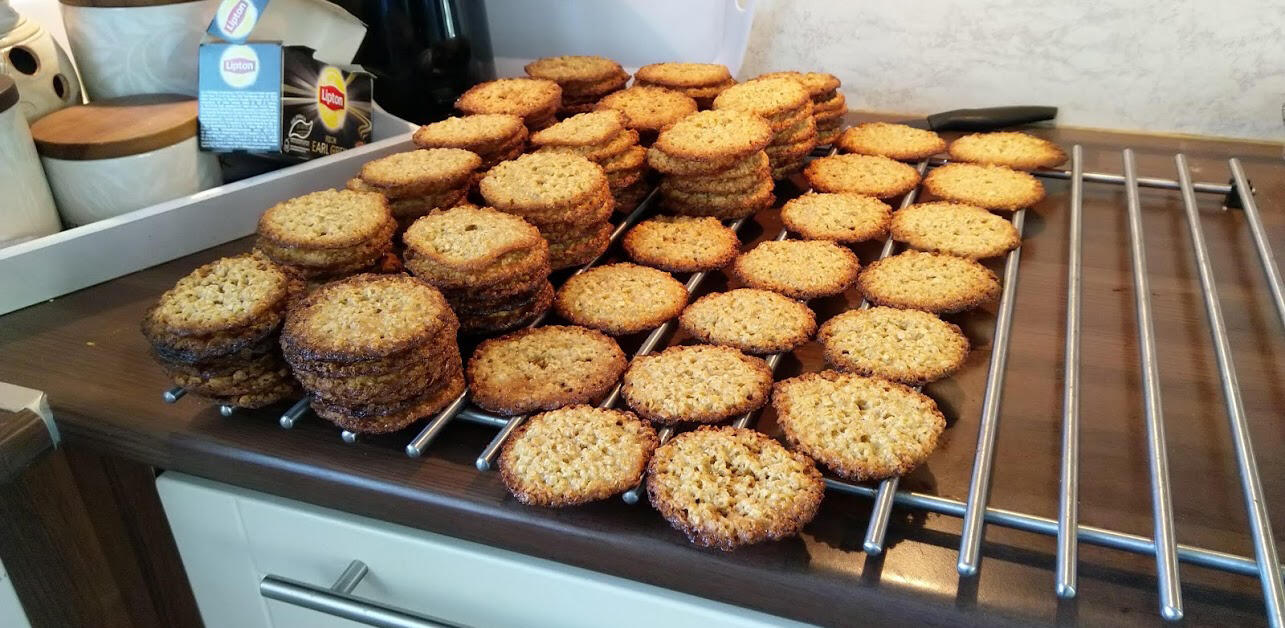
\includegraphics[height=\textheight]{havreflarn/IMG_20190711_151829.jpg}}
    \end{figure}

%    \introduction{
%
%	}

	\ingredients[6]{
		\SI{7}{\tablespoon} & Butter \\
		\SI{1}{\cup} & Sugar \\
		\SI{3}{\tablespoon} & Flour \\
		\SI{1x3/4}{\cup} & Rolled oats \\
		\SI{2}{\teaspoon} & Baking powder \\
		2 & Eggs
	}

	\preparation{
		\step Preheat oven to \SI{400}{\fahrenheit} (\SI{205}{\celsius}).

		\vspace{1em}

		\step Melt \SI{7}{\tablespoon} of butter in a pan.

		\vspace{1em}

		\step Mix sugar, flour, oats, and baking powder in a bowl until well combined.

		\step Add 2 eggs to bowl and mix.

		\vspace{1em}

		\step Add melted butter to bowl and mix until fully combined.

		\vspace{1em}

		\step Cover baking trays or cookie sheets with parchment paper.

		\vspace{1em}

		\step Plop down cookie batter onto trays/sheets in balls about 1 tablespoon at a time, leaving plenty of space between each cookie-to-be.

		\step Bake for \SIrange{6}{8}{\minute}, until cookie is flat, golden, and brown around the edges.
	}

\end{recipe}